\documentclass{article}
\usepackage{amsmath}
\usepackage{amssymb}
\usepackage{graphicx}
\usepackage{hyperref}
\usepackage[version=4]{mhchem}


\begin{document}
\section*{Problem}
In triangle \(A B C, \angle C=90^{\circ} . \angle 1=\angle 2 . C D: B D=3: 5\). Find \(B C\) if \(A B\) \(=10 \mathrm{~mm}\).\\
\centering
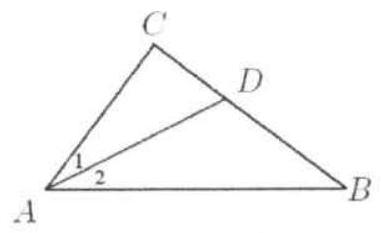
\includegraphics[width=\textwidth]{images/064(1).jpg}

\section*{Solution}
8 mm .\\
Draw \(D E \perp A B\) so that the perpendicular line meets \(A B\) at \(E . \triangle C A D\) and \(\triangle A E D\) are congruent and \(D E=C D\).\\
Since \(\angle B=\angle B, \angle B E D=\angle C=90^{\circ}, \triangle B D E \sim \triangle B A C\).\\
So \(\frac{D E}{A C}=\frac{B D}{A B} \Rightarrow \quad \frac{D E}{B D}=\frac{A C}{A B}\).\\
Since \(C D: B D=3: 5, \frac{D E}{B D}=\frac{3}{5} \Rightarrow \frac{A C}{A B}=\frac{3}{5}\).\\
\centering
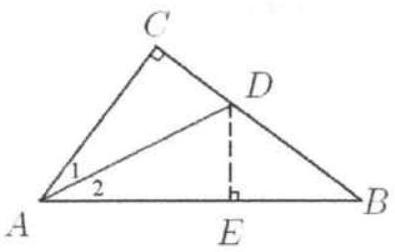
\includegraphics[width=\textwidth]{images/067.jpg}

Since \(A B=10, A C=6\).\\
\(B C=\sqrt{A B^{2}-A C^{2}}=\sqrt{10^{2}-6^{2}}=8\).

\end{document}
